% Options for packages loaded elsewhere
\PassOptionsToPackage{unicode}{hyperref}
\PassOptionsToPackage{hyphens}{url}
%
\documentclass[
]{article}
\usepackage{amsmath,amssymb}
\usepackage{iftex}
\ifPDFTeX
  \usepackage[T1]{fontenc}
  \usepackage[utf8]{inputenc}
  \usepackage{textcomp} % provide euro and other symbols
\else % if luatex or xetex
  \usepackage{unicode-math} % this also loads fontspec
  \defaultfontfeatures{Scale=MatchLowercase}
  \defaultfontfeatures[\rmfamily]{Ligatures=TeX,Scale=1}
\fi
\usepackage{lmodern}
\ifPDFTeX\else
  % xetex/luatex font selection
\fi
% Use upquote if available, for straight quotes in verbatim environments
\IfFileExists{upquote.sty}{\usepackage{upquote}}{}
\IfFileExists{microtype.sty}{% use microtype if available
  \usepackage[]{microtype}
  \UseMicrotypeSet[protrusion]{basicmath} % disable protrusion for tt fonts
}{}
\makeatletter
\@ifundefined{KOMAClassName}{% if non-KOMA class
  \IfFileExists{parskip.sty}{%
    \usepackage{parskip}
  }{% else
    \setlength{\parindent}{0pt}
    \setlength{\parskip}{6pt plus 2pt minus 1pt}}
}{% if KOMA class
  \KOMAoptions{parskip=half}}
\makeatother
\usepackage{xcolor}
\usepackage[margin=1in]{geometry}
\usepackage{color}
\usepackage{fancyvrb}
\newcommand{\VerbBar}{|}
\newcommand{\VERB}{\Verb[commandchars=\\\{\}]}
\DefineVerbatimEnvironment{Highlighting}{Verbatim}{commandchars=\\\{\}}
% Add ',fontsize=\small' for more characters per line
\usepackage{framed}
\definecolor{shadecolor}{RGB}{248,248,248}
\newenvironment{Shaded}{\begin{snugshade}}{\end{snugshade}}
\newcommand{\AlertTok}[1]{\textcolor[rgb]{0.94,0.16,0.16}{#1}}
\newcommand{\AnnotationTok}[1]{\textcolor[rgb]{0.56,0.35,0.01}{\textbf{\textit{#1}}}}
\newcommand{\AttributeTok}[1]{\textcolor[rgb]{0.13,0.29,0.53}{#1}}
\newcommand{\BaseNTok}[1]{\textcolor[rgb]{0.00,0.00,0.81}{#1}}
\newcommand{\BuiltInTok}[1]{#1}
\newcommand{\CharTok}[1]{\textcolor[rgb]{0.31,0.60,0.02}{#1}}
\newcommand{\CommentTok}[1]{\textcolor[rgb]{0.56,0.35,0.01}{\textit{#1}}}
\newcommand{\CommentVarTok}[1]{\textcolor[rgb]{0.56,0.35,0.01}{\textbf{\textit{#1}}}}
\newcommand{\ConstantTok}[1]{\textcolor[rgb]{0.56,0.35,0.01}{#1}}
\newcommand{\ControlFlowTok}[1]{\textcolor[rgb]{0.13,0.29,0.53}{\textbf{#1}}}
\newcommand{\DataTypeTok}[1]{\textcolor[rgb]{0.13,0.29,0.53}{#1}}
\newcommand{\DecValTok}[1]{\textcolor[rgb]{0.00,0.00,0.81}{#1}}
\newcommand{\DocumentationTok}[1]{\textcolor[rgb]{0.56,0.35,0.01}{\textbf{\textit{#1}}}}
\newcommand{\ErrorTok}[1]{\textcolor[rgb]{0.64,0.00,0.00}{\textbf{#1}}}
\newcommand{\ExtensionTok}[1]{#1}
\newcommand{\FloatTok}[1]{\textcolor[rgb]{0.00,0.00,0.81}{#1}}
\newcommand{\FunctionTok}[1]{\textcolor[rgb]{0.13,0.29,0.53}{\textbf{#1}}}
\newcommand{\ImportTok}[1]{#1}
\newcommand{\InformationTok}[1]{\textcolor[rgb]{0.56,0.35,0.01}{\textbf{\textit{#1}}}}
\newcommand{\KeywordTok}[1]{\textcolor[rgb]{0.13,0.29,0.53}{\textbf{#1}}}
\newcommand{\NormalTok}[1]{#1}
\newcommand{\OperatorTok}[1]{\textcolor[rgb]{0.81,0.36,0.00}{\textbf{#1}}}
\newcommand{\OtherTok}[1]{\textcolor[rgb]{0.56,0.35,0.01}{#1}}
\newcommand{\PreprocessorTok}[1]{\textcolor[rgb]{0.56,0.35,0.01}{\textit{#1}}}
\newcommand{\RegionMarkerTok}[1]{#1}
\newcommand{\SpecialCharTok}[1]{\textcolor[rgb]{0.81,0.36,0.00}{\textbf{#1}}}
\newcommand{\SpecialStringTok}[1]{\textcolor[rgb]{0.31,0.60,0.02}{#1}}
\newcommand{\StringTok}[1]{\textcolor[rgb]{0.31,0.60,0.02}{#1}}
\newcommand{\VariableTok}[1]{\textcolor[rgb]{0.00,0.00,0.00}{#1}}
\newcommand{\VerbatimStringTok}[1]{\textcolor[rgb]{0.31,0.60,0.02}{#1}}
\newcommand{\WarningTok}[1]{\textcolor[rgb]{0.56,0.35,0.01}{\textbf{\textit{#1}}}}
\usepackage{graphicx}
\makeatletter
\def\maxwidth{\ifdim\Gin@nat@width>\linewidth\linewidth\else\Gin@nat@width\fi}
\def\maxheight{\ifdim\Gin@nat@height>\textheight\textheight\else\Gin@nat@height\fi}
\makeatother
% Scale images if necessary, so that they will not overflow the page
% margins by default, and it is still possible to overwrite the defaults
% using explicit options in \includegraphics[width, height, ...]{}
\setkeys{Gin}{width=\maxwidth,height=\maxheight,keepaspectratio}
% Set default figure placement to htbp
\makeatletter
\def\fps@figure{htbp}
\makeatother
\setlength{\emergencystretch}{3em} % prevent overfull lines
\providecommand{\tightlist}{%
  \setlength{\itemsep}{0pt}\setlength{\parskip}{0pt}}
\setcounter{secnumdepth}{-\maxdimen} % remove section numbering
% definitions for citeproc citations
\NewDocumentCommand\citeproctext{}{}
\NewDocumentCommand\citeproc{mm}{%
  \begingroup\def\citeproctext{#2}\cite{#1}\endgroup}
\makeatletter
 % allow citations to break across lines
 \let\@cite@ofmt\@firstofone
 % avoid brackets around text for \cite:
 \def\@biblabel#1{}
 \def\@cite#1#2{{#1\if@tempswa , #2\fi}}
\makeatother
\newlength{\cslhangindent}
\setlength{\cslhangindent}{1.5em}
\newlength{\csllabelwidth}
\setlength{\csllabelwidth}{3em}
\newenvironment{CSLReferences}[2] % #1 hanging-indent, #2 entry-spacing
 {\begin{list}{}{%
  \setlength{\itemindent}{0pt}
  \setlength{\leftmargin}{0pt}
  \setlength{\parsep}{0pt}
  % turn on hanging indent if param 1 is 1
  \ifodd #1
   \setlength{\leftmargin}{\cslhangindent}
   \setlength{\itemindent}{-1\cslhangindent}
  \fi
  % set entry spacing
  \setlength{\itemsep}{#2\baselineskip}}}
 {\end{list}}
\usepackage{calc}
\newcommand{\CSLBlock}[1]{\hfill\break\parbox[t]{\linewidth}{\strut\ignorespaces#1\strut}}
\newcommand{\CSLLeftMargin}[1]{\parbox[t]{\csllabelwidth}{\strut#1\strut}}
\newcommand{\CSLRightInline}[1]{\parbox[t]{\linewidth - \csllabelwidth}{\strut#1\strut}}
\newcommand{\CSLIndent}[1]{\hspace{\cslhangindent}#1}
\ifLuaTeX
  \usepackage{selnolig}  % disable illegal ligatures
\fi
\usepackage{bookmark}
\IfFileExists{xurl.sty}{\usepackage{xurl}}{} % add URL line breaks if available
\urlstyle{same}
\hypersetup{
  pdftitle={LDP\_manuscript},
  pdfauthor={Katherine Gyte},
  hidelinks,
  pdfcreator={LaTeX via pandoc}}

\title{LDP\_manuscript}
\author{Katherine Gyte}
\date{2024-09-15}

\begin{document}
\maketitle

Microalgae form colonies in response to predator grazing, but they also
form larger aggregates in response to prolonged or more severe
environmental stressors (Lürling 2003). Roccuzzo et al. (2020) found
that the aggregation behaviour of microalgae requires an investment in
fatty acid metabolism.

\textbf{Methods}

\emph{Experimental setup}

Cultures of \emph{Tetradesmus obliquus} in COMBO media (CPCC 5, Canadian
Phycological Culture Centre, University of Waterloo, Canada) were
exposed to three different experimental concentrations of microplastics
(MP): ``low'' (100MP/mL; 4mg/L, n=4), ``medium'' (1,000MP/mL; 40mg/L,
n=4), and ``high'' (10,000MP/mL; 400mg/L, n=4). Treatment cultures were
assembled in 50mL Falcon Tubes containing approximately 4 million algal
cells and with 0.004\% Tween20. Experimental treatments were incubated
at 24ºC under a 12:12 light:dark cycle for 15 days. Samples for analysis
were collected on Day 1, Day 12, and Day 15.

\emph{Data collection}

On days 1, 12, and 15 of the experiment, samples from each biological
replicate (n=4) were taken and the number and size of algal aggregates
were measured using a FlowCam 8400 machine with the corresponding
VisualSpreadsheet software (Version 6, Fluid Imaging Technologies). A
100um FlowCell and a 10x objective lens were used, while the FlowCam
context settings were set to 0.1mL/min flow rate (approx. 50\%
efficiency) with 4um minimum threshold particle size for imaging.

\emph{Aggregation behaviour analysis}

Changes in aggregation behaviour were measured based on the proportion
of algal aggregates in the total population. To differentiate single
algal cells from stacked algal colonies and from algal aggregates, the
FlowCam imaging data was sorted by convex perimeter which was visually
ascertained to be the parameter that best separated cells, stacks, and
aggregates. To further sort the aggregates from the rest of the data, a
threshold convex perimeter of 80um was chosen, again based on visual
analysis of the imaging data. The total number of images collected by
the FlowCam correspond to the total cell count of the sample, and the
number of images above the 80um convex perimeter threshold correspond to
the number of aggregates present in the sample.

To standardise differences in total cell count between samples, the
proportion of algal aggregates (calculated by dividing the number of
aggregates by the total cell count for each sample) was compared across
treatments. Data collected on days 12 and 15 were also normalised to day
1 counts. A linear mixed effects model (Proportion aggregate
\textasciitilde{} Treatment + (1\textbar Replicate)) was run to
determine any statistical differences across microplastic treatments.

\textbf{Results}

\emph{Algal aggregation behaviour}

Changes in \emph{T. obliquus} aggregation behaviour were measured across
microplastic concentrations by calculating the mean proportion of
aggregates in algal cultures across treatments. Importantly, the
presence of the Tween20 surfactant alone did not have an effect on the
proportion aggregate compared to the control without the Tween20
surfactant added (ANOVA, p \textgreater{} 0.05) (Fig. 1).

Interestingly, samples collected on Day 1 of the experiment (hours after
adding the microplastics to algal cultures) showed a rapid and dose
dependent response to the microplastic treatments (Fig. 1).

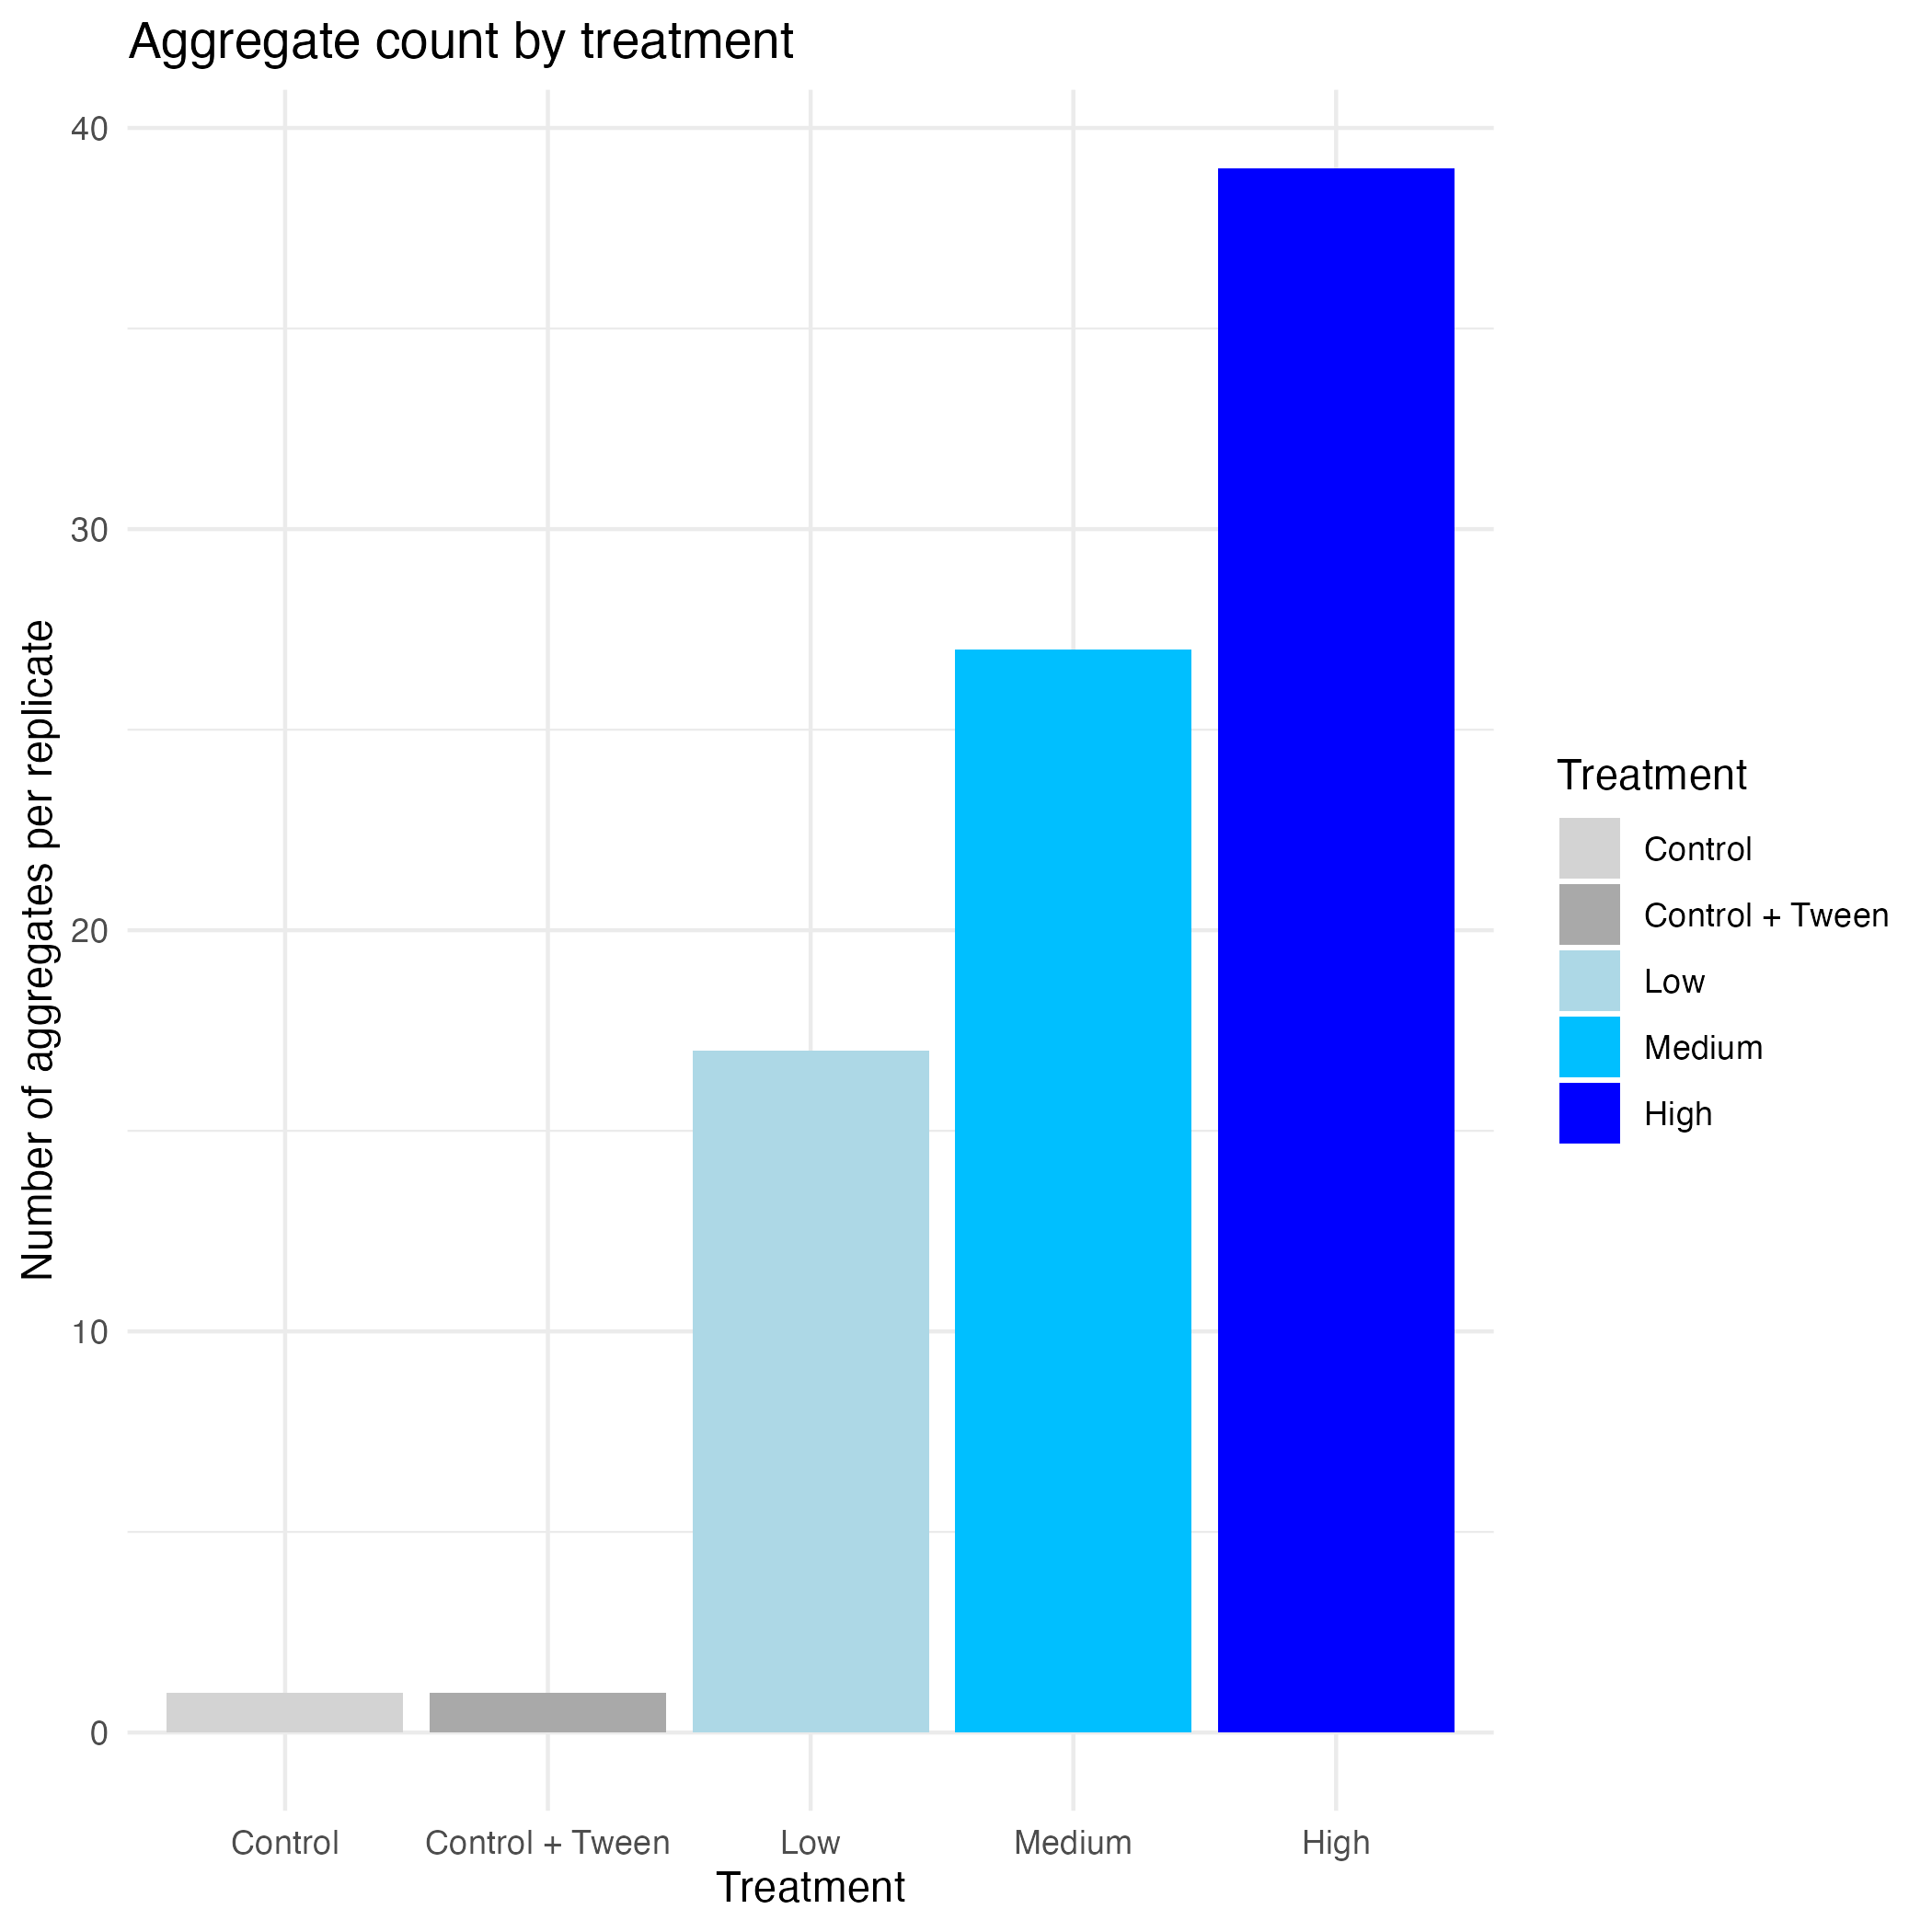
\includegraphics{03_figures/D1_agcount.png} Figure 1. Bar plot showing
the number of algal aggregates across microplastic treatments.

\emph{Algal aggregate size}

In addition to increasing the number of aggregates, exposure to higher
concentrations of microplastics also increased the size of the algal
aggregates in culture. Based on the FlowCam imaging data, the area of
particles captured could be measured to provide information on changes
to aggregate size across treatments. We found that aggregate area
increased with microplastic concentration (Fig. 2).

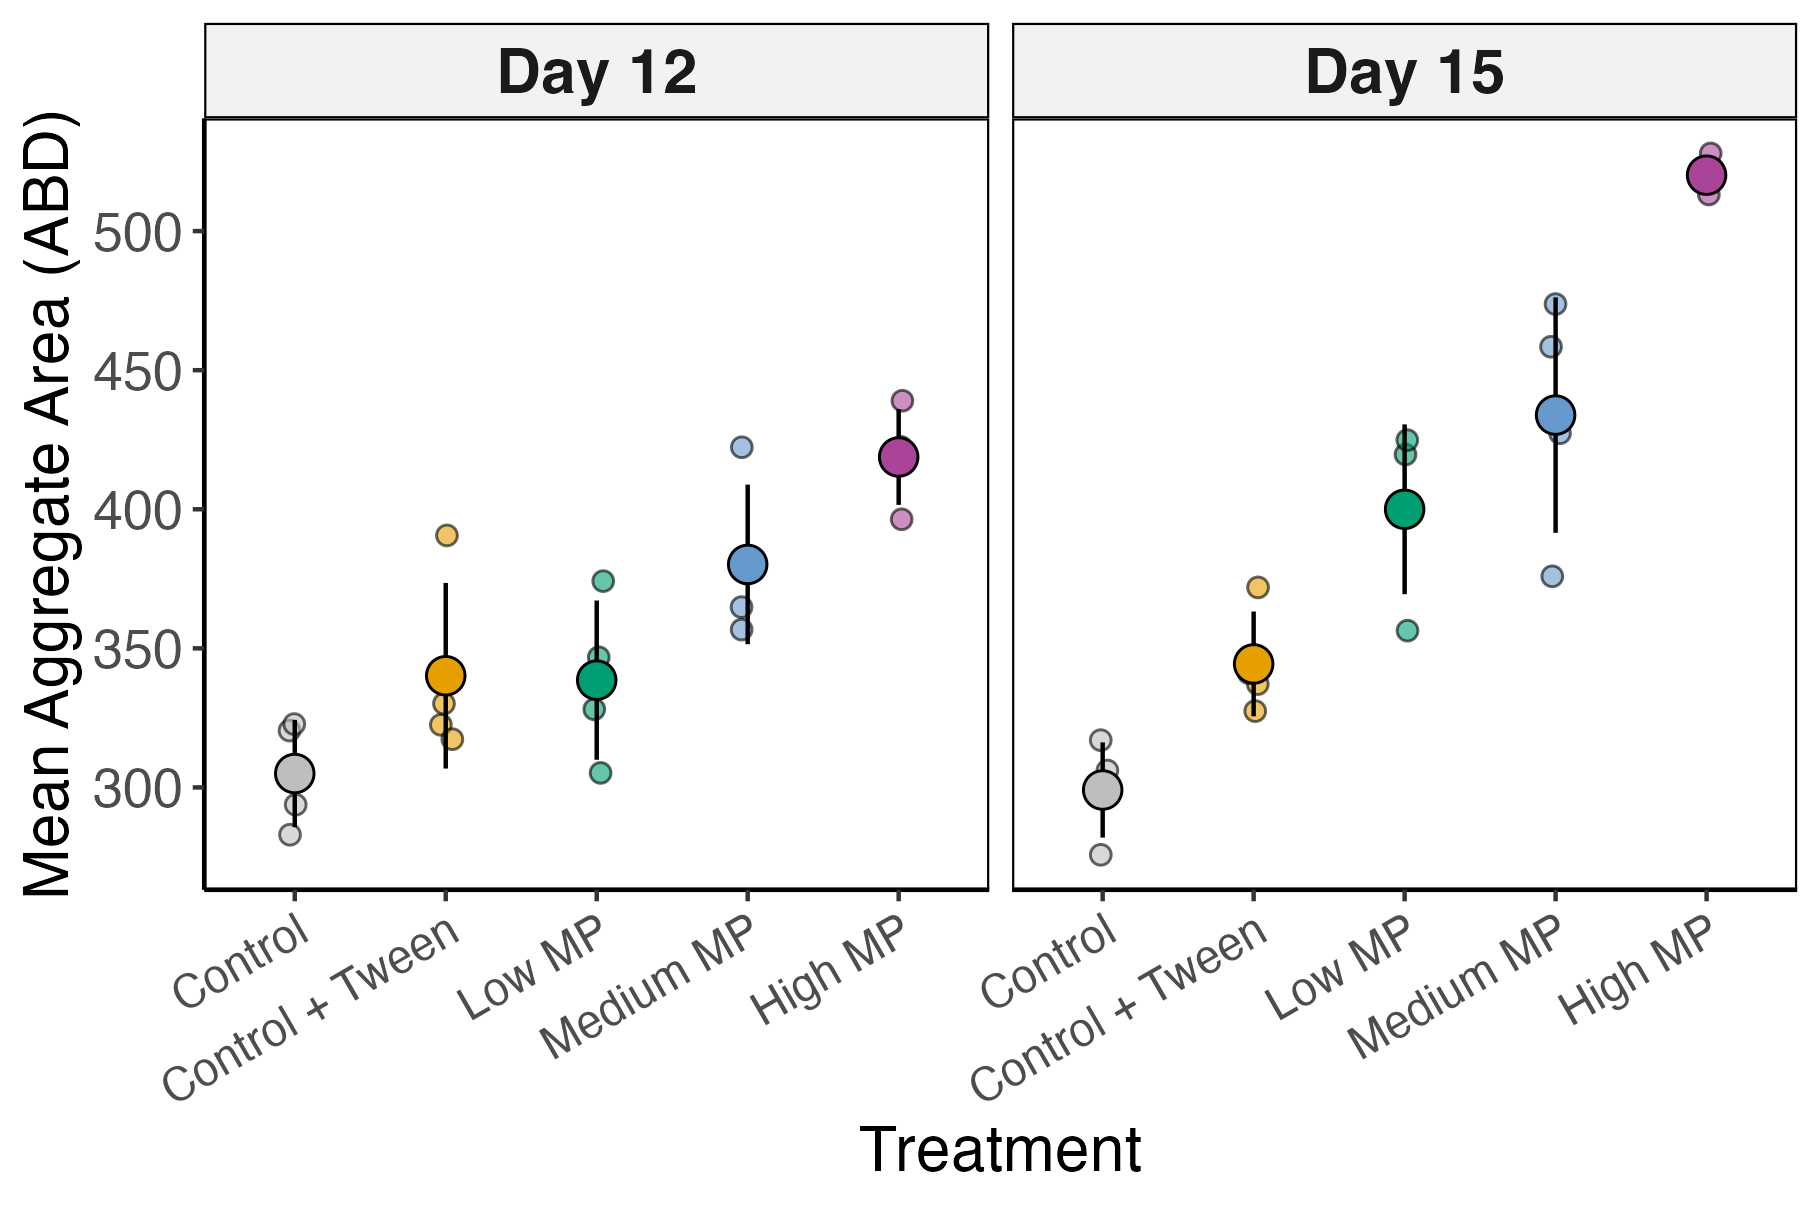
\includegraphics{03_figures/nod1.agg.area.png} Figure 2. Area of
microalgal aggregates across microplastic treatment groups.

\begin{Shaded}
\begin{Highlighting}[]
\NormalTok{grateful}\SpecialCharTok{::}\FunctionTok{cite\_packages}\NormalTok{(}\AttributeTok{output =} \StringTok{"paragraph"}\NormalTok{, }\AttributeTok{out.dir =} \StringTok{"."}\NormalTok{)}
\end{Highlighting}
\end{Shaded}

We used R version 4.4.1 (\textbf{base?}) and the following R packages:
here v. 1.0.1 (\textbf{here?}), prereg v. 0.6.0 (\textbf{prereg?}), renv
v. 1.0.7 (\textbf{renv?}), rmarkdown v. 2.27 (\textbf{rmarkdown2018?};
\textbf{rmarkdown2020?}; \textbf{rmarkdown2024?}), tidyverse v. 2.0.0
(\textbf{tidyverse?}), trackdown v. 1.1.1 (\textbf{trackdown?}).

\phantomsection\label{refs}
\begin{CSLReferences}{1}{0}
\bibitem[\citeproctext]{ref-luxfcrling2003}
Lürling, M. 2003. {``Phenotypic Plasticity in the Green Algae
Desmodesmus and Scenedesmus with Special Reference to the Induction of
Defensive Morphology.''} \emph{Annales de Limnologie - International
Journal of Limnology} 39 (2): 85--101.
\url{https://doi.org/10.1051/limn/2003014}.

\bibitem[\citeproctext]{ref-roccuzzo2020}
Roccuzzo, Sebastiana, Narciso Couto, Esther Karunakaran, Rahul Vijay
Kapoore, Thomas O. Butler, Joy Mukherjee, Erika M. Hansson, Andrew P.
Beckerman, and Jagroop Pandhal. 2020. {``Metabolic Insights into
Infochemicals Induced Colony Formation and Flocculation in Scenedesmus
Subspicatus Unraveled by Quantitative Proteomics.''} \emph{Frontiers in
Microbiology} 11 (May). \url{https://doi.org/10.3389/fmicb.2020.00792}.

\end{CSLReferences}

\end{document}
